\section{An intro chap on motivation and experiments?}
\begin{itemize}
  \item Time crystals?
  \item Time-resolved diffraction patters, temporal double slit experiment + Muga theory \url{https://arxiv.org/pdf/0812.3034.pdfß}
\end{itemize}

%\clearpage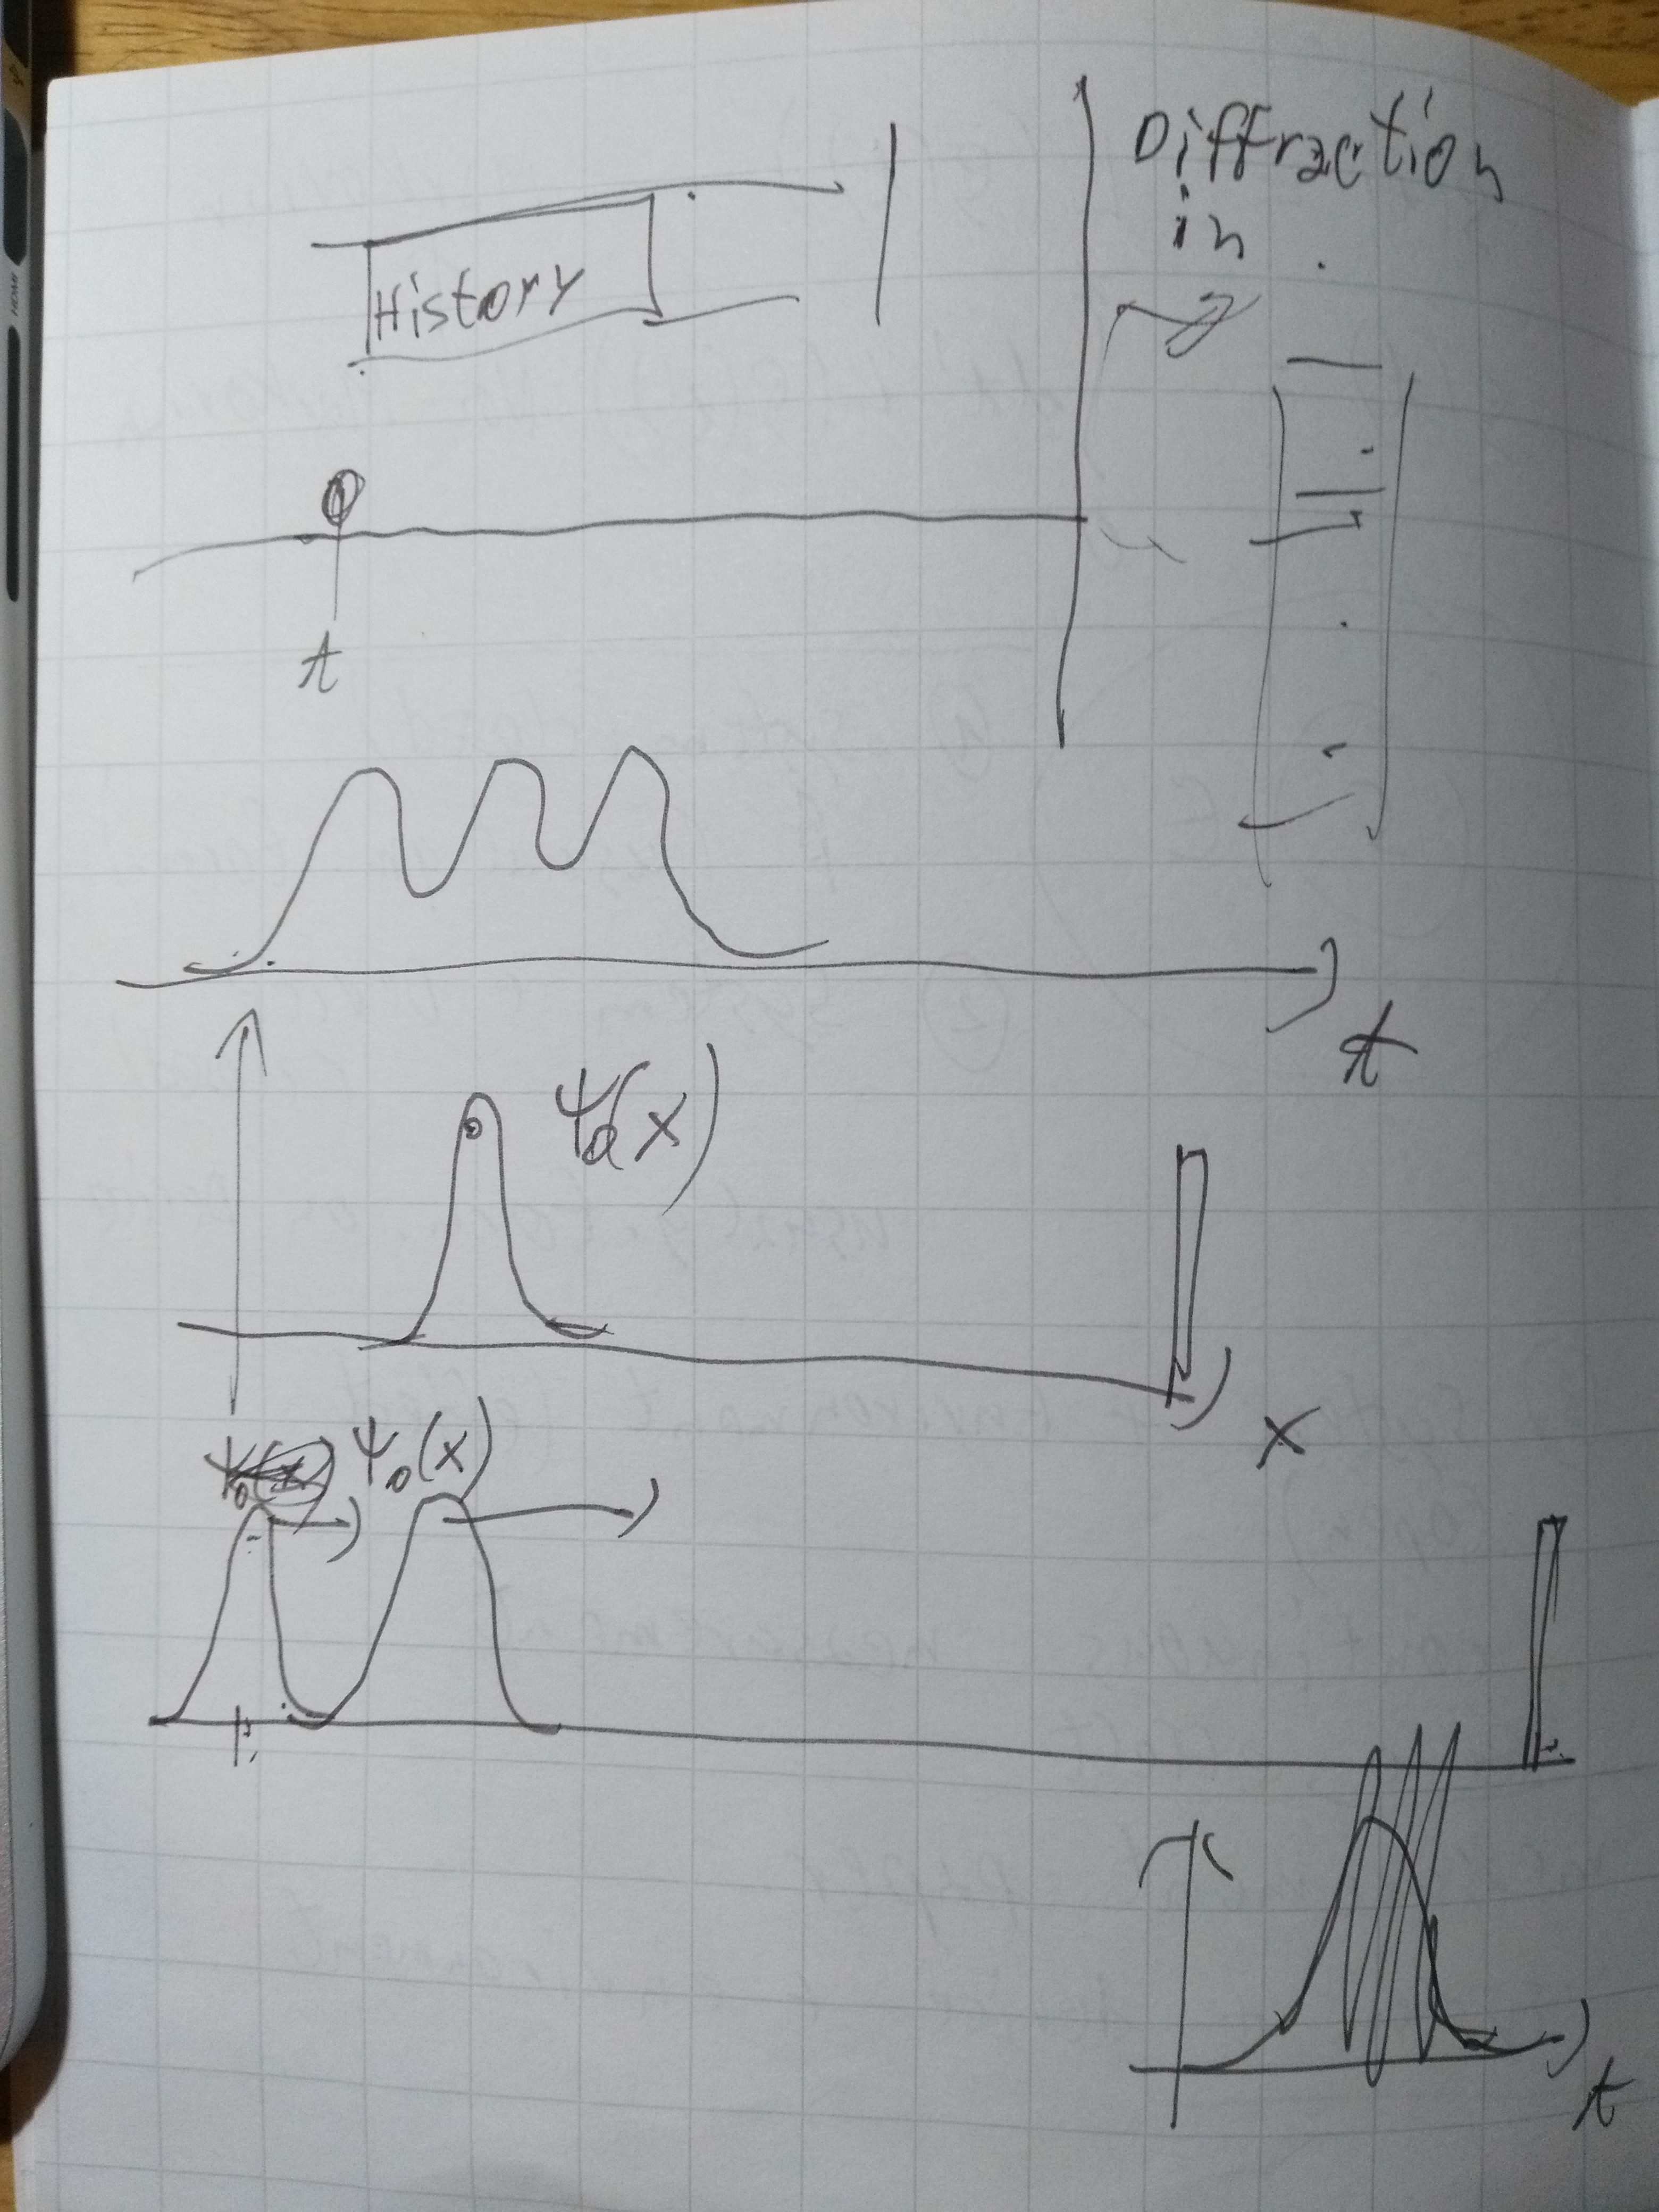
\includegraphics[width=\linewidth]{img/diffraction.jpg}


\section{Time crystals}

References: \cite{crystal2,crystal3,crystal2012}.


\section{Irrev}
\subsection{Use open quantum systems theory in ``Decoherence and measurement'' chapter}
Schmidt decompositions, spatial and temporal states in
$\hilb{H}_T$ and $\hilb{H}_S$
are described as density operators
(mixed states). What if there isn't a ``perfect entanglment'' between space and time.

\section{Entanglement and decoherence (Arrow of time)}
See also \cite{EntanglementVsDecoherence}.

Decoherence is an irreversible process, it also happens in measurement.

According to Marletto and Vedral, arrow of time is increase in Entanglement
between the clock and the rest.

So, there seems to be a contradiction: is entanglement ``decreasing''
(i.e. destroyed by decoherence) with time
or increasing?

We can avoid the contradiction saying that
entanglement between two finite systems is
destroyed while the entanglement of each of them with the universe
is increasing.

\subsection{``Harmonic clocks''}

TODO: use the harmonic oscillator in \cite{HarmonicClocks}
as a PaW clock for the same packet that is measured in
Ruschhaupt's detector model.

Therein, fading wave function: is minus derivative an event?
L4 normalized?


\subsection{Misc}

Idea: use section B ``Measurement'' of \cite{Lloyd:Time}: detector as (binary) measument device.

``Philospher'': \url{https://arxiv.org/abs/1704.07236}.

Time of arrival and clocks: again, \cite{YearsleyHalliwell_Clocks}.
Which maybe suggests we should not wory too much of $H\ket{\Psi} = 0$. 

We don't. 

BUT please note \cite{YearsleyHalliwell_Clocks} uses a clock that is
\emph{coupled} with the system, while in PaW they are ``only'' entangled.
So their calculation may be unnecessarily complicated.
Maybe the weakjly coupling case can be used?

Other systems of interest: decays. Prvanovic new.

Reference \cite{ConnesRovelliThermo}.

Relate with John Goold's works? The ancilla as a clock? --- Topical Review

Markovianity, histories.

Lloyd on arXiv: from clock to cloners; erasing; scrambling (as in Goold).

Lloyd on decoherent histories (Gellman, Hartle?).

Dechoerence / irreversibility / measurement.

Vedral / Lloyd. Discord.

Measuring entanglement: Quantification of Concurrence via Weak Measurement: 1611.00149.

Marletto/Vedral on Arrow of time. Arrow of time as increasing entanglement.

Arrow of time: 

\url{https://www.wired.com/2014/04/quantum-theory-flow-time/}

\url{https://en.wikipedia.org/wiki/Loschmidt%27s_paradox}

\url{https://www.quantamagazine.org/20160119-time-entanglement/}

\url{https://arxiv.org/pdf/1702.07706.pdf} \textit{The second law of thermodynamics at the microscopic scale}
Thibaut Josset,
Aix Marseille Univ. (David).

Maxwell's demon: https://arxiv.org/pdf/1702.05161.pdf

\subsection{and paths}

Both \cite{YearsleyHalliwell_Clocks} and \cite{Gambini_PW}
reason in terms of paths and actions, maybe Feynmann stuff
in following chapter... and maybe conistent historiesapproach can help
towards linking PaW and ToA?

Also \url{http://quantum.phys.cmu.edu/CHS/CHS_transp.pdf}.

\subsection{Decays?}

We might want to look at exponential decay from \url{https://arxiv.org/abs/1704.07236},
then compare with exponential decay with P and W using Lloyd Giovannetti and Maccone (ref).

\subsubsection{Purification}

See https://arxiv.org/pdf/quant-ph/0512125.pdf, P-W time as a purifying ancilla
of the (Kijowski?) time.

\section{Misc/Multi/Extras/TODO/Outlook}

\url{https://arxiv.org/abs/1703.05876}
--- \emph{comment}: time measured and stored here
may be all classical information
so this paper may or may not be relevant for the topic.

But
``prototypes of clocks based on quantum principles,
such as entanglement and squeezing''
may make this interesting again, see reference therein.
They also cite Lloyd, Giovannetti and Maccone,
but a paper quite older than \cite{Lloyd:Time}.

\url{https://arxiv.org/abs/1603.02522}
\emph{Decoherence by spontaneous emission: a single-atom analog of superradiance}.
Decoherent histories, non-markovianity, open quantum systems.

\url{https://arxiv.org/abs/1007.2615} Time travel / Quantum CTC.

Carmichael et al. \cite{CarmichaelOQS2017} (Andreas's reading)
(non-markovianity).

Non-markovian, quantum-to-classical, open systems, David,
\url{https://arxiv.org/pdf/1703.09428.pdf}.

In his works, Zurek mentions:
DeWitt, Everett, gell_Mann, hartl, Many Worlds, consistent/decoherent histories:
idea: Lagrangian over a history? Principle of least action?

Zurek: ``Reduction of the Wavepacket: How Long Does it Take?'' (arxiv),
``quantum''' time? \cite{Zurek_Einselect} also mentions
``decoherence timescale''.

Von Neumann/Shannon entropy in measurement? Mention information problems
in quantum cosmology (where a quantum time is necessary)? Etc. etc.
